%\documentclass[12pt,aps,pra,showkeys,nofootinbib,notitlepage,groupedaddress]{revtex4-1}
\documentclass{article}
\usepackage{header}

\begin{document}

\makeatletter
\title{Lightning Stokes Solver}
\author{Pablo Brubeck \and Nick Trefethen}
\date{\today}
\makeatother

\maketitle

\begin{abstract}
Gopal and Trefethen have recently introduced ``lightning solvers''
for the 2D Laplace and Helmholtz equations, based on rational
functions with poles exponentially clustered near singular corners.
Making use of the Goursat representation in terms of analytic
functions, we extend these methods to the biharmonic equation,
specifically to 2D Stokes flow.  Flows in bounded, unbounded, and
multiply connected domains are considered, with solutions computed
to ten digits of accuracy in a few seconds of laptop time.  As an
illustration of the high accuracy, we readily resolve two or three
counter-rotating Moffatt eddies near a singular corner.
\end{abstract}

\linespread{1}
%!TEX root = stokes_paper.tex

\section{Introduction}

In this paper we consider numerical solutions to the biharmonic equation in a two-dimensional domain $\Omega\subseteq\reals^2$,
\begin{equation} \label{eq:bih}
\nabla^4 \psi = \nabla^2 \left(\nabla^2 \psi\right) = \psi_{xxxx} +2\psi_{xxyy} +\psi_{yyyy} = 0,
\end{equation}
coupled with appropriate boundary conditions. Since the equation is of fourth order, to ensure
well-posedness, we impose two boundary conditions at each point of $\partial\Omega$. We specify the value of
the function itself and one component of the gradient on a portion $\Gamma_1$ of $\partial\Omega$, and both components
of the gradient on the complementary part $\Gamma_2$ ,
\begin{subequations}\label{eq:bcs}
\begin{equation}
\psi = h(x,y), \quad \uvec{a}\cdot \nabla\psi = k(x,y)\quad \text{on }\Gamma_1,\\
\end{equation}
\begin{equation}
\nabla \psi = \vec{g}(x,y) \quad\text{on }\Gamma_2,
\end{equation}
\end{subequations}
where $\uvec{a}\in\reals^2$ is a fixed unit vector, with $\partial\Omega = \Gamma_1 \cup \Gamma_2$ and $\Gamma_1\cap\Gamma_2 = \emptyset$. Functions that satisfy \eqref{eq:bih} are called biharmonic and are smooth in the interior of $\Omega$, although point-singularities may arise on the boundary when $\partial\Omega$ contains corners or when the boundary data $h$, $k$, $\vec{g}$ have singularities, or at points of juncture between $\Gamma_1$ and $\Gamma_2$.

In this paper, we propose a numerical method to solve \eqref{eq:bih}--\eqref{eq:bcs} by generalizing the recently introduced ``lightning solvers'' for the 2D Laplace and Helmholtz equations \cite{gopal19,gopal19new}. The main advantage of this class of methods is that they can handle very general singularities in very general domains with corners, without requiring any detailed analysis, and still achieve high accuracy.

This work is structured as follows. In Section \ref{sec:goursat}, we describe the Goursat representation, which allows one to write any solution to \eqref{eq:bih} in terms of two analytic functions when $\Omega$ is simply connected. These two functions can then be approximated by rational functions \cite{newman64}.
The biharmonic equation is most commonly found in applications in Stokes flow and linear elasticity. In Section \ref{sec:physics}, we review how the incompressible Stokes equations can be represented
via the stream function, which is biharmonic. For linear elasticity problems, one transforms the governing equations into a biharmonic equation involving the Airy stress function, but problems
of elasticity are not explored in this paper.


Our method consists of approximating both Goursat functions by rational functions and finding coefficients that best satisfy the boundary conditions \eqref{eq:bcs} in the least-squares sense. A detailed description of the method, along with implementation details, is given in Section \ref{sec:method}, and numerical results are presented in Section \ref{sec:results}. The method gets high accuracy for simple geometries with great speed, and we illustrate this by showing its ability to easily resolve two or more Moffatt eddies in corners. In Section \ref{sec:unbounded}, we show how to extend the method to unbounded domains directly without the need for artificial boundaries. Section  \ref{sec:multiply} presents an extension to multiply connected regions by the inclusion of additional logarithmic terms. Finally, we give our
conclusions in Section \ref{sec:conclusion}.
%!TEX root = stokes_paper.tex
\newtheorem{theorem}{Theorem}

\section{Biharmonic functions in simply-connected domains \label{sec:goursat}}

The Goursat representation is the key ingredient required to extend the lightning solver to biharmonic problems, going back to the French mathematician Goursat in 1898 \cite{goursat}. It allows one to represent biharmonic functions in terms of two analytic functions, which our algorithms will then approximate by rational functions. In line with the use of analytic functions, and throughout the rest of the paper, we represent $x$ and $y$ via the complex variable $z = x + iy$. We include a precise statement of the Goursat representation in the form of a theorem, along with two proofs, which we consider to be valuable in giving two perspectives on what is going on. The original proof was given by Goursat in \cite{goursat}, and an alternative proof is given by Muskhelishvili in \cite{mus19}. Both of these are also found in textbooks such as \cite{ockendon95} and \cite{mus77}. Although we label them ``proofs'', we don’t give these arguments in full detail. For a rigorous discussion, see [\textbf{Find a reference for this}].


\begin{theorem}[Goursat representation]
\label{th:goursat}
Let $\Omega\subseteq\mathbb{C}$ be a simply-connected open region, and let
$\psi : \Omega \rightarrow \reals$ be a biharmonic function. Then $\psi$ can be represented in terms of functions $f(z)$ and $g(z)$ analytic in $\Omega$ by the formula
\begin{equation}\label{eq:goursat}
\psi(x,y) = \psi(z,\conj{z}) = \Im \left\{ \conj{z}f(z) + g(z)\right\}.
\end{equation}
The functions $f(z)$ and $g(z)$ are uniquely defined up to addition of arbitrary terms $\lambda z+C$ to $f(z)$ and $\conj{C}z+\alpha$ to $g(z)$, where $\lambda,\alpha\in\reals$ and $C\in\mathbb{C}$.
\end{theorem}

The use of the imaginary as opposed to the real part is standard in the literature and helps
to simplify the expressions for physical quantities associated with $\psi$. Series expansions based on
\eqref{eq:goursat} have been used to find numerical solutions to BVPs associated with \eqref{eq:bih} by Gaskell et al. in
\cite{gaskell}, Finn, Cox and Byrne in \cite{finn}, and by Luca and Crowdy in \cite{luca18}, among many others. Though
the Goursat representation has been used by various people over the years, it is used far less than more general tools such as FEM and integral equations and indeed is surprisingly hard to find in textbooks.


\begin{proof}[Goursat's proof \cite{Gou98}]
First, we note that the biharmonic operator can be written in terms of Wirtinger derivatives,
\begin{equation}
\nabla^4 \psi = 16\frac{\partial^4 \psi}{\partial\conj{z}^2 \partial z^2}.
\end{equation}
Treating $z$ and $\conj{z}$ as independent variables, one can solve this equation by separation of variables. Under the assumption that $\psi$ is analytic with respect to te real variables $x$ and $y$, we may plug in the ansatz $\psi=\sum_k \psi_k$, where $\psi_k= A_k(z)B_k(\conj{z})$, obtaining
\begin{equation}
\frac{\partial^4 \psi_k}{\partial\conj{z}^2 \partial z^2} = A_k''(z) B_k''(\conj{z}) = 0,
\end{equation} 
which implies that either $A_k''(z)=0$ or $B_k''(\conj{z})=0$. The solution spaces for these two cases are spanned by $\{1,z\}$ for $A_k''(z)=0$  and $\{1,\conj{z}\}$ for $B_k''(\conj{z})=0$. Therefore, without loss of generality, by superposition of the four independent solutions,
\begin{equation}
\psi(z,\conj{z}) =  A_1(z) + \conj{z} A_2(z) + B_3(\conj{z}) + z B_4(\conj{z}),
\end{equation}
where $A_1(z), A_2(z), B_3(\conj{z}), B_4(\conj{z})$ are arbitrary functions. Since $\psi$ must be real, $\psi=\conj{\psi}$ implies that 
\begin{equation}
\psi(z,\conj{z}) =  A_1(z)  + \conj{z} A_2(z)  + \conj{A_1(z)} + z \conj{A_2(z)} = 2 \Re\left\{A_1(z) + \conj{z} A_2(z)\right\},
\end{equation}
which implies \eqref{eq:goursat} by letting $f(z) = -2i A_2(z)$ and $g(z) = -2i A_1(z)$. We finally note that, when $\psi$ is given, $f(z)$ and $g(z)$ are determined up to an additive linear term. To be more precise, the substitutions $f(z)\to f(z)+\lambda z + C$ together with $g(z)\to g(z)+\conj{C}z+\alpha$ for $\lambda,\alpha\in\reals$ and $C\in\mathbb{C}$ leave $\psi$ invariant.
\end{proof}


\begin{proof}[Muskhelishvili's proof \cite{Mus19}]
If $\omega=-\nabla^2 \psi$, then $-\nabla^2\omega = \nabla^4\psi = 0$. Now define $p$ as the harmonic conjugate of $\omega$, satisfying the Cauchy-Riemann conditions
\begin{equation}
\frac{\partial\omega}{\partial x} = \frac{\partial p}{\partial y}, \quad
\frac{\partial\omega}{\partial y} = -\frac{\partial p}{\partial x};
\end{equation}
this function is determined up to an arbitrary constant, $p_0\in\reals$. Then the expression
\begin{equation}
h(z) = p(x,y)-i\omega(x,y)
\end{equation}
represents a function of the complex variable $z=x+iy$, analytic in $\Omega$. Put
\begin{equation}
f(z) := \frac{1}{4} \int_a^z h(w) dw = f_1 + if_2,
\end{equation}
where $a\in\Omega$ is arbitrary, causing $f(z)$ to be defined up to a term $\lambda z +C$ where $4\lambda=p_0$ and $C\in\mathbb{C}$. Obviously,
\begin{equation}\label{eq:fprime}
f'(z) = \frac{\partial f_1}{\partial x} + i \frac{\partial f_2}{\partial x} = -i \frac{\partial f_1}{\partial y} + \frac{\partial f_2}{\partial y} = \frac{1}{4} \left(p-i\omega\right),
\end{equation}
from which, we calculate, using the fact that $\nabla^2 f_1=\nabla^2 f_2=0$,
\begin{equation}
\nabla^2\left(y f_1\right) = 2\frac{\partial f_1}{\partial y} = \frac{\omega}{2},\quad \nabla^2\left(x f_2\right) = 2\frac{\partial f_2}{\partial x} = -\frac{\omega}{2}.
\end{equation}
Thus, the function $\psi + yf_1 - xf_2$ is harmonic, since
\begin{equation}
\nabla^2 \left(\psi + yf_1 - xf_2\right) = -\omega + \frac{\omega}{2} + \frac{\omega}{2} =0.
\end{equation}
Let this function be $\psi + yf_1 - xf_2 = \Im\left\{g(z)\right\}$, where $g(z)$ is analytic, and for the given $f(z)$, it will be defined up to a term $\conj{C}z+\alpha$, where $\alpha\in\reals$, since $\psi$ must not depend on the term $C\conj{z}$. Hence one can represent
\begin{equation}
\psi = x f_2(z) -y f_1(z) + \Im\left\{g(z)\right\} = \Im\left\{\conj{z}f(z) + g(z)\right\}.
\end{equation}
This argument can be used to establish the analyticity of $\psi$.
\end{proof}
%!TEX root = stokes_paper.tex

\section{Physical interpretation: Stokes flow}

Let $\vec{u}=(u,v)^T$ be the velocity field of a steady incompressible 2D fluid flow, and let $p$ be the associated pressure field, which is defined up to a constant. In the limit $\text{Re}\to 0$ and in the absence of body forces, the steady-state equations for the conservation of momentum and the incompressibility constraint are given by
\begin{subequations}\label{eq:stokes}
\begin{align}
-\nabla^2 \vec{u} + \nabla p &= 0,\label{eq:momen}\\
\nabla\cdot\vec{u} &= 0. \label{eq:incomp}
\end{align}
\end{subequations}
A common solution technique is to introduce the stream function $\psi$ by letting
\begin{equation}
u=\frac{\partial\psi}{\partial y}, \quad 
v=-\frac{\partial\psi}{\partial x}.
\end{equation}
Then, it is easy to verify that \eqref{eq:incomp} is automatically satisfied. Now define the vorticity as
\begin{equation}
\omega := \frac{\partial v}{\partial x} - \frac{\partial u}{\partial y}  = -\nabla^2 \psi.
\end{equation}
Note that \eqref{eq:momen} takes the form of the Cauchy-Riemann conditions 
\begin{equation}\label{eq:pomega}
-\nabla^2u=\frac{\partial\omega}{\partial y} = -\frac{\partial p}{\partial x} , \quad 
-\nabla^2v=-\frac{\partial\omega}{\partial x} = -\frac{\partial p}{\partial y},
\end{equation}
which directly imply that $p$ and $\omega$ are harmonic conjugates. Therefore, the stream function-vorticity formulation
\begin{subequations}
\begin{align}
-\nabla^2\psi &= \omega,\label{eq:psi}\\
-\nabla^2\omega &= 0,\label{eq:omega}
\end{align}
\end{subequations}
is equivalent to the system of equations \eqref{eq:stokes}. Moreover, one can take the Laplacian on both sides of \eqref{eq:psi} and use \eqref{eq:omega} to reveal that $\psi$ is biharmonic. Thus we have reduced the original system of three equations in three unknowns to a biharmonic equation. By Theorem \ref{th:goursat}, one can write
\begin{equation}
\psi = \frac{1}{2i} \left[g(z) - \conj{g(z)} + \conj{z}f(z) - z\conj{f(z)}\right].
\end{equation}
so that the velocity components are given in terms of $f(z)$ and $g(z)$,
\begin{equation}
u-iv = 2i\frac{\partial \psi}{\partial z} = g'(z) + \conj{z} f'(z) - \conj{f(z)}.
\end{equation}
Since $\psi$ is invariant under the transformations of Theorem \ref{th:goursat}, so are $u$ and $v$. The vorticity is then given by
\begin{equation}
-\omega = \nabla^2 \psi =4\frac{\partial^2\psi}{\partial \conj{z}\partial z} = -2i \left( f'(z) - \conj{f'(z)}\right) = 4\Im\left\{f'(z)\right\},
\end{equation}
and from \eqref{eq:pomega} we deduce that
\begin{equation}
p-i\omega = 4 f'(z).
\end{equation}
Since the pressure is uniquely defined up to a constant, we can relate this freedom to a pressure shift of $p_0=4\lambda$. 


Let us further introduce the Airy stress function $A$, which we will define as the biharmonic conjugate of $-2\psi$, implying that $-2(p-i\omega) = \nabla^2 (A-2i\psi)$


a potential for the stress tensor $\sigma_{ij} = u_{i,j} + u_{j,i} -p \delta_{ij}$,
\begin{equation}
\matlabmatrix{\sigma_{11} \sigma_{12}; \sigma_{21} \sigma_{22}} = 
\matlabmatrix{A_{yy} -A_{xy}; -A_{yx} A_{xx}}.
\end{equation}
Since only second derivatives of $A$ have a physical interpretation, $A$ is uniquely defined up to a linear term. We can connect the three corresponding degrees of freedom with those on the arbitrariness on the Goursat representation, defined as the biharmonic conjugate of $\psi$,
\begin{equation}\label{eq:stress}
-\frac{A}{2}+i\psi := \conj{z}f(z) + g(z).
\end{equation}
We note that \eqref{eq:stress} can be transformed into
\begin{equation}
-\frac{A}{2}+i\psi = \conj{z}f(z) + g(z) + \left(\lambda \conj{z}z + C\conj{z} + \conj{C}z + \alpha \right), 
\end{equation}
without changing the physical description of the fluid. From the terms in parenthesis, we observe that only $\lambda \conj{z}z$ has an effect on the stress tensor, namely the pressure shift. The rest of these terms are of the form $c_1 x+c_2 y+\alpha$ which coincides with the arbitrariness in the definition of $A$, and correspond to rigid-body displacements.


\subsection{Moffatt eddies}

The asymptotic solution ($r \ll r_0$) for the anti-symmetric flow inside a wedge of angle $2\alpha$ caused by a perturbation at infinity was studied by Moffat in \cite{Moffatt64},
\begin{equation}
\psi_\lambda(r,\theta) \sim \Re\left\{\left(\frac{r}{r_0}\right)^\lambda \left[\cos{(\lambda\alpha)}\cos{\left((\lambda-2)\theta\right)}+\cos{\left((\lambda-2)\alpha\right)}\cos{(\lambda\theta)}\right]\right\},
\end{equation}
where, in order to satisfy the no-slip conditions $\psi_\lambda=\uvec{n}\cdot\nabla\psi_\lambda=0$ at $\theta=\pm\alpha$, the parameter $\lambda$ must be a root of
\begin{equation}\label{eq:roots}
\sin{\left(2\alpha(\lambda-1)\right)} + (\lambda-1)\sin{(2\alpha)}=0.
\end{equation}
If $2\alpha>146^\circ$, the non-trivial roots of \eqref{eq:roots} are complex, $\lambda=p + iq$, which means that $\psi_\lambda$ presents radial oscillations (periodic in $\log(r)$) of decaying amplitude at a rate of $r^{p}$, which is manifested as a sequence of counter-rotating vortices, commonly known as Moffat eddies.


%!TEX root = stokes_paper.tex

\section{Method and Algorithm}

\subsection{Rational functions}
Following Gopal and Trefethen \cite{Gopal19}, we use rational functions to approximate the analytic functions in the Goursat representation, which warranties a biharmonic function, hence we only need to find the coefficients that best fit the boundary conditions, we do this via least-squares.
\begin{equation}
f(z) = \sum_{k=1}^N f_j \phi_j(z), \quad g(z) = \sum_{k=1}^N g_j \phi_j(z),
\end{equation}
where 
\begin{equation}
\left\{\phi_j(z)\right\}_{j=1}^{N} = \left\{p_k(z)\right\}_{k=0}^{N_1} \cup \left\{\frac{1}{z/\beta_k-1}\right\}_{k=1}^{N_2}
\end{equation}
where the $p_k(z)$ are the discretely-orthogonal ``Vandermonde with Arnoldi'' polynomials from \cite{Brubeck19}, which obey the $k+2$-term recurrence relation
\begin{equation}
H_{k,k+1} p_{k+1}(z) = z p_k(z) - \sum_{j=0}^k H_{j,k} p_j(z),\quad k=1,\ldots,N_1, \quad p_0(z)=1.
\end{equation}
with $H$ being the upper Hessenberg matrix from the Arnoldi iteration on the Krylov subspace $\mathcal{K}_{N_1}(\diag(z_i), e)$, where $e$ is the vector with all entries equal to 1. And the poles $\beta_k$ are clustered near the corners of $\Omega$, $\left\{w_n\right\}_{n=1}^P$, as described in \cite{Gopal19},
\begin{equation}
\beta_{k,n} = w_n + Le^{i\theta_n} e^{-\sigma (\sqrt{M_n}-\sqrt{k})}, \quad k=1,\ldots,M_n,\quad n=1,\ldots,P,
\end{equation}
where $\sigma=4$, $\theta_n$ is the angle formed between the real axis and the angle bisector at the corner $w_n$, and $L$ is some characteristic length scale associated with $\Omega$.









\subsection{Matrix system}


The enforcement of boundary conditions at the sample points $z_k$ is carried on by approximately solving by least-squares
\begin{equation} \label{eq:LS}
A x\approx b,
\end{equation}
where $A\in\reals^{2M\times 4N}$, $x\in\reals^{4N}$ and $b\in\reals^{2M}$. If we partition the system into blocks, each associating the complex coefficients for a basis function $\phi_j(z)$ where the point $z_k$ where it or its derivative are evaluated, we obtain
\begin{equation}
\matlabmatrix{A_{11} {\cdots} A_{1N}; {\vdots} {\ddots} {\vdots}; A_{M1} {\cdots} A_{MN}}
\matlabmatrix{x_{1}; {\vdots}; x_{N}} \approx \matlabmatrix{b_{1}; {\vdots}; b_{M}},
\end{equation}
where $A_{kj}\in\reals^{2\times 4}$ are the blocks associated with the basis function $\phi_{j}(z)$ evaluated at $z=z_i$, $b_k\in\reals^2$ correspond to the RHS for the two BCs imposed at $z=z_k$, and $x_j\in\reals^4$ contain the 4 real DoFs of the complex coefficients of $\phi_j(z)$ in $f(z)$ and $g(z)$
\begin{equation}
x_ j = \matlabmatrix{\real{f_j} \imag{f_j} \real{g_j} \imag{g_j}}^\transp.
\end{equation}



For instance, a condition on both velocity components imposed at $z=z_k$ will correspond to two rows with RHS $b_k=(U(z_k), -V(z_k))^\transp$ and blocks
\begin{equation}
A_{kj}=\matlabmatrix{\real{\conj{z_k}\phi'_j(z_k)-\phi_j(z_k)} -\imag{\conj{z_k}\phi'_j(z_k)-\phi_j(z_k)} \real{\phi'_j(z_k)} -\imag{\phi'_j(z_k)}; 
\imag{\conj{z_k}\phi'_j(z_k)+\phi_j(z_k)} \phantom{+}\real{\conj{z_k}\phi'_j(z_k)+\phi_j(z_k)} \imag{\phi'_j(z_k)} \phantom{+}\real{\phi'_j(z_k)}},
\end{equation}
for $j=1,\ldots,N$. A no-slip condition can be implemented by providing a zero RHS.
For a slip condition, one may also specify the velocity component tangential and set the stream function to some constant $C$ along the boundary. At the point $z=z_k$, this will correspond to two rows with RHS $b_k=(U_t(z_k),C)^\transp$ and blocks
\begin{equation}
A_{kj}=\matlabmatrix{\imag{F_{kj}} \real{F_{kj}} \imag{G_{kj}} \real{G_{kj}}; 
\imag{\conj{z_k}\phi_j(z_k)} \real{\conj{z_k}\phi_j(z_k)} \imag{\phi_j(z_k)} \real{\phi_j(z_k)}},
\end{equation}
for $j=1,\ldots,N$, where $F_{kj}=e^{i\alpha_k}\conj{z_k}\phi'_j(z_k)+e^{-i\alpha_k}\phi_j(z_k)$,  $G_{kj}=e^{i\alpha_k}\phi'_j(z_k)$, and $\alpha_k$ denotes the angle between the vector normal to the boundary and the real axis.

In our implementation, we solve \eqref{eq:LS} with MATLAB's backslash. But in order to get good results, it is crucial to do column scaling, which we do by right preconditioning with
\begin{equation}
D=\diag( A^\transp A)^{-1/2}.
\end{equation} 
This can be illustrated in a few lines of code,.
\begin{verbatim}
D = spdiag(1./sqrt(sum(A.^2,1)));
y = (A*D)\b; 
x = D*y;
\end{verbatim}


\subsection{Adaptive refinement}
We use a similar adaptive refinement strategy to the one that is presented in \cite{Gopal19}, which is producing a sequence of linear least-squares problems of increasing size. In brief, we associate each entry of the residual vector with the nearest corner by defining the index sets
\begin{equation}
\mathcal{I}_k = \left\{1\leq j\leq N : \arg\min_{1\leq i \leq M} \abs{w_i-z_j}=k\right\},\quad k=1,\ldots, P.
\end{equation}
And after solving the least-squares problem, we decide to increase the number of poles based on the partial residuals, 
\begin{equation}
R_k^2 = \sum_{j\in \mathcal{I}_k} r_j^2,\quad k=1,\ldots, P,
\end{equation}
on which we do a histogram. On the next least-squares problem, we increase the number of poles on every corner, but more poles will be placed near the corners that fall on the bin with the largest residual.


\subsection{The algorithm}
Here is our algorithm for solving \eqref{eq:bvp}. 

\begin{algorithm}[H]
	\SetAlgoLined
	Define boundary $\partial \Omega$, corners $w_1,\ldots,w_P$, boundary function $h$ and tolerance $\varepsilon$\;
	\While{True}{
		Define rational function basis\;
		Choose sampling points $z_i$, clustered near corners\;
		Form the matrix $A$ and RHS vector $b$\;
		Solve the least-squares problem $Ax\approx b$ for the coefficient vector $x$\;
		Exit loop if $\norm{Ax-b}_2<\varepsilon$ or if $N$ too large or if the error is growing\;
		Form the residual histogram and increment the number of poles per corner\;
	}
	Confirm accuracy by checking error on a finer boundary mesh\;
	Construct a function to evaluate the solution based on the computed coefficiets $x$\;
	\caption{The lightning Stokes solver.}
\end{algorithm}

%!TEX root = ../main.tex

\section{Results}

\begin{frame}
\frametitle{A smooth problem: Moffatt eddies inside a wedge}
\centering
\begin{figure}
	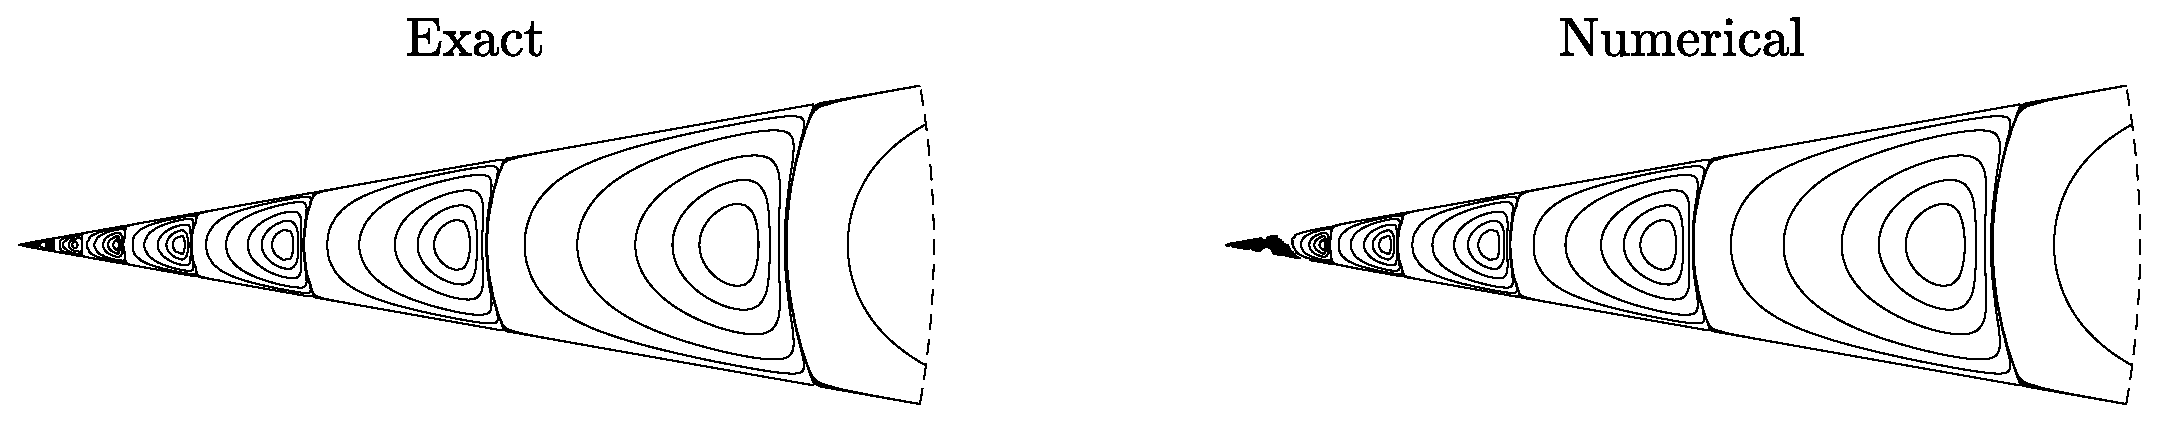
\includegraphics[width=\linewidth]{Figures/moff_psi}
	
	\vfill
	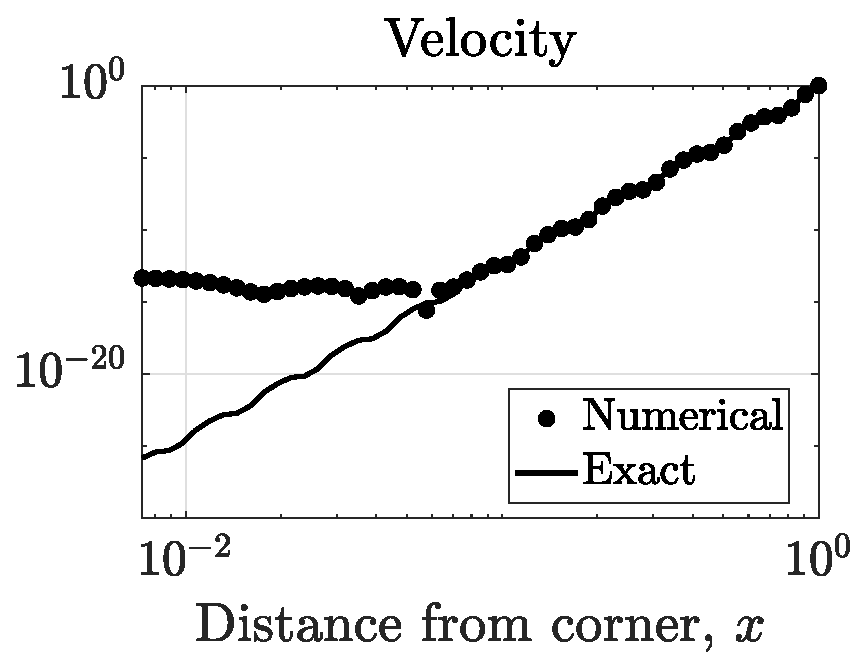
\includegraphics[height=0.3\linewidth]{Figures/moff_vel}
	\hfill
	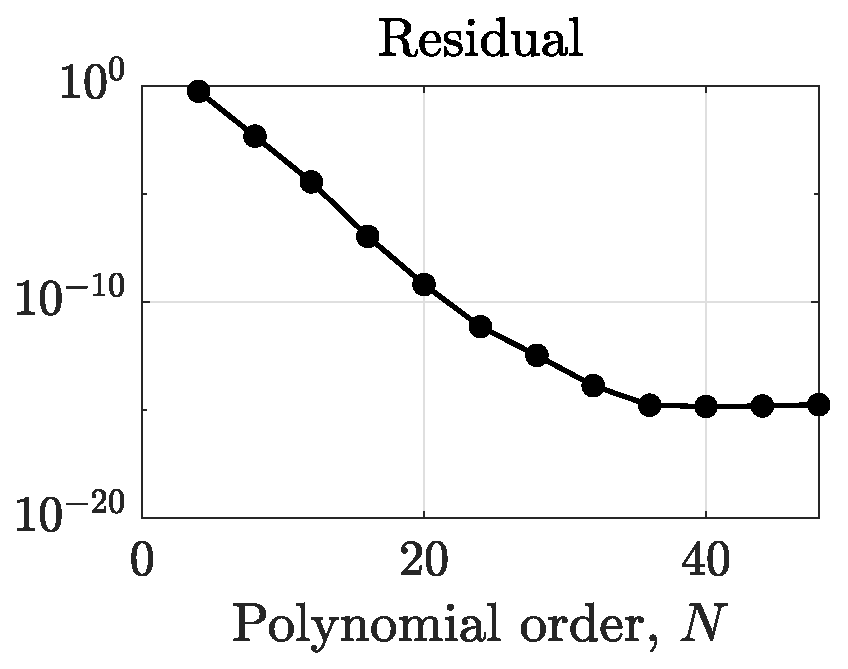
\includegraphics[height=0.3\linewidth]{Figures/moff_res}
\end{figure}

\end{frame}


\begin{frame}
\frametitle{Discontinuous boundary data: lid-driven cavity}
\centering
\begin{figure}
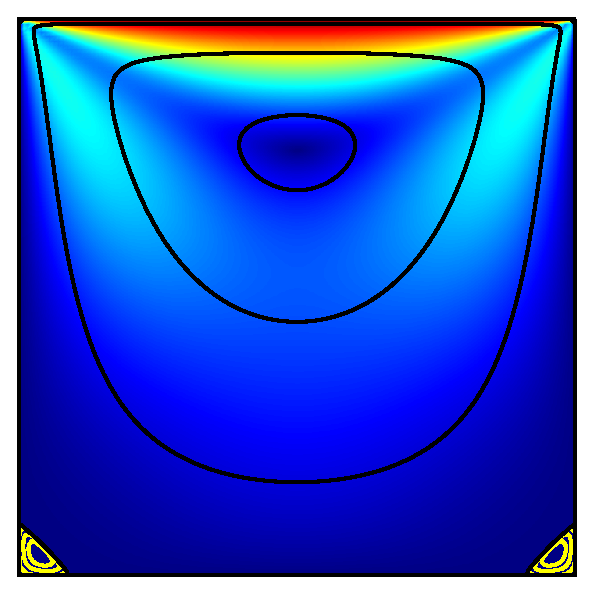
\includegraphics[height=0.5\linewidth]{Figures/ldc_soln}
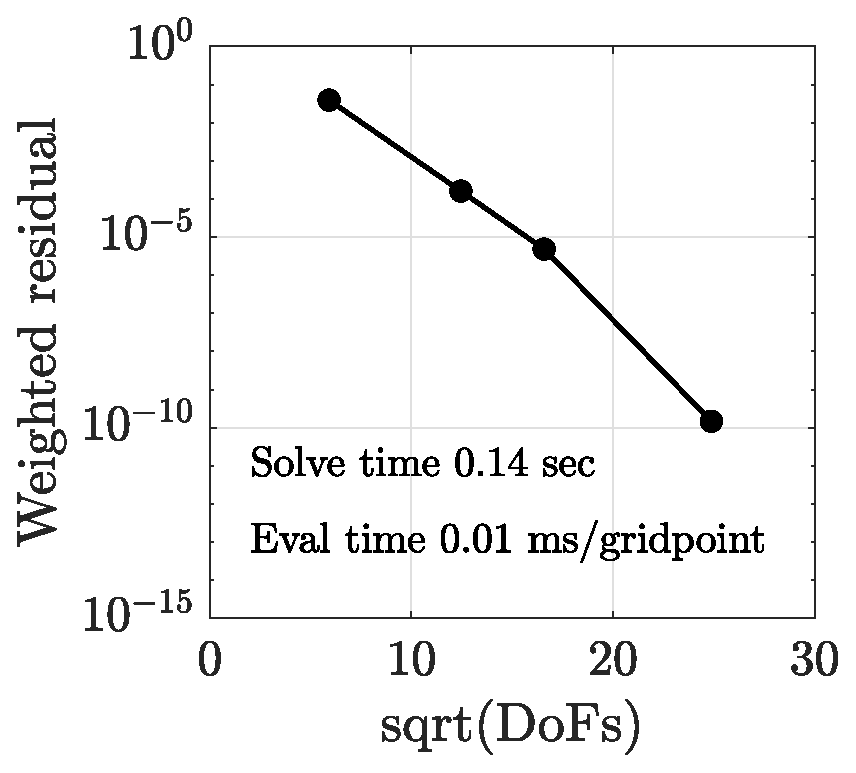
\includegraphics[height=0.4\linewidth]{Figures/ldc_conv}
\end{figure}
\end{frame}



\begin{frame}
\frametitle{Re-entrant corner: backwards-facing step}
\centering
\begin{figure}
	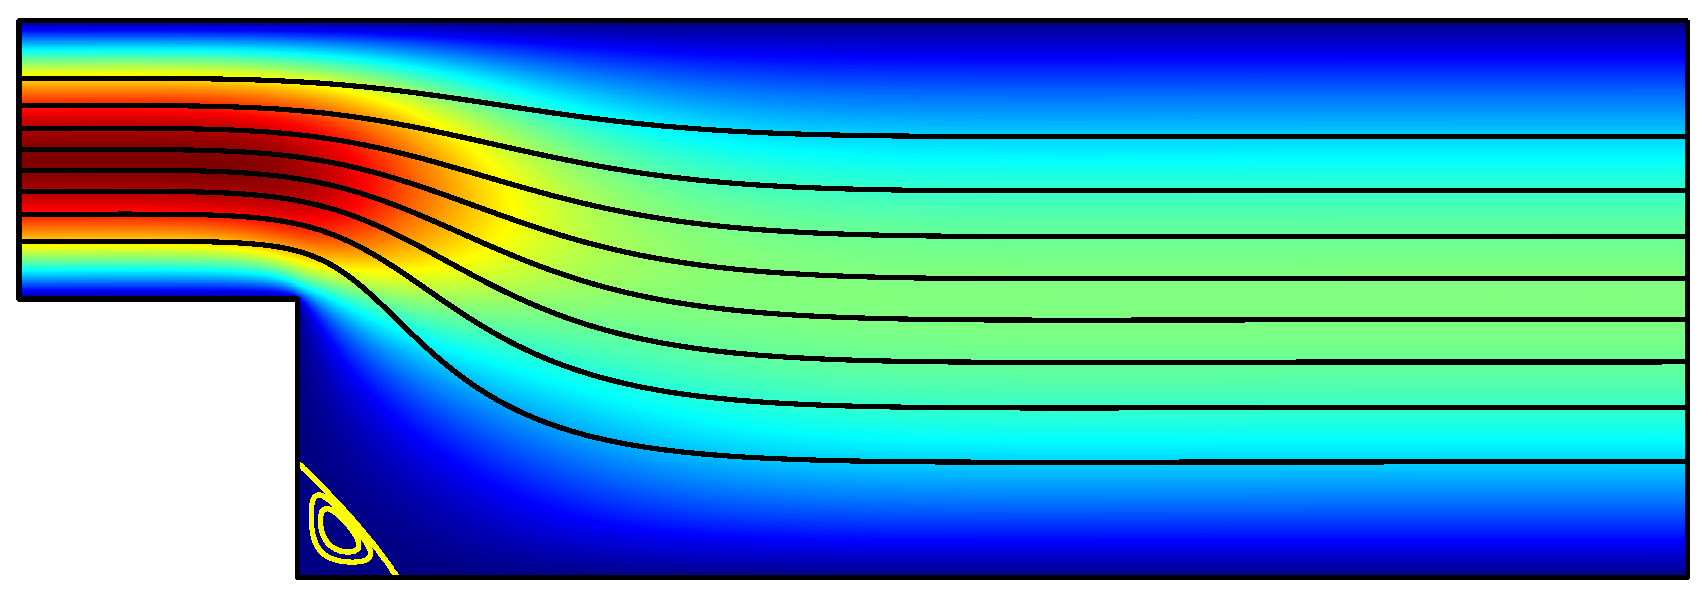
\includegraphics[height=0.3\linewidth]{Figures/step_soln}
	
	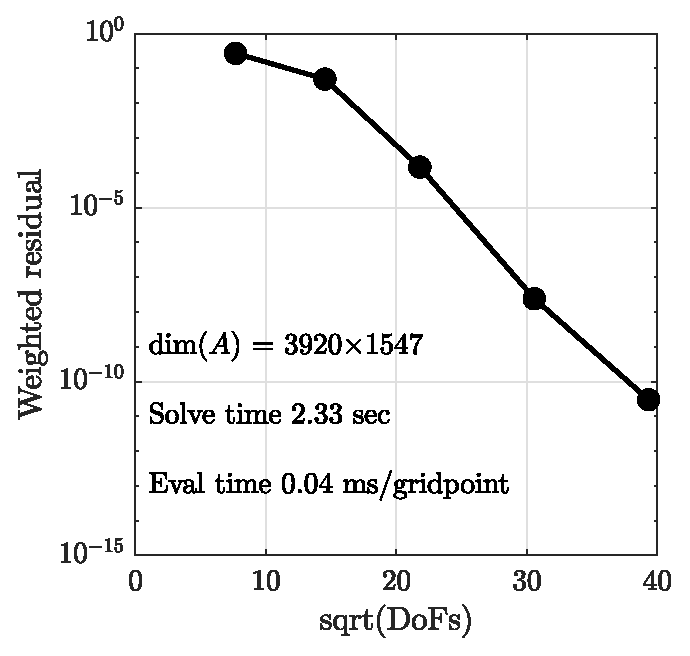
\includegraphics[height=0.3\linewidth]{Figures/step_conv}
\end{figure}
\end{frame}


\begin{frame}
\frametitle{Infinitely long backwards-facing step}
\centering
\begin{figure}
	%\captionsetup{position=top}
	\subcaptionbox*{$-\infty\xleftarrow{\hspace*{0.4\linewidth}}x\xrightarrow{\hspace*{0.4\linewidth}}\infty$}{
		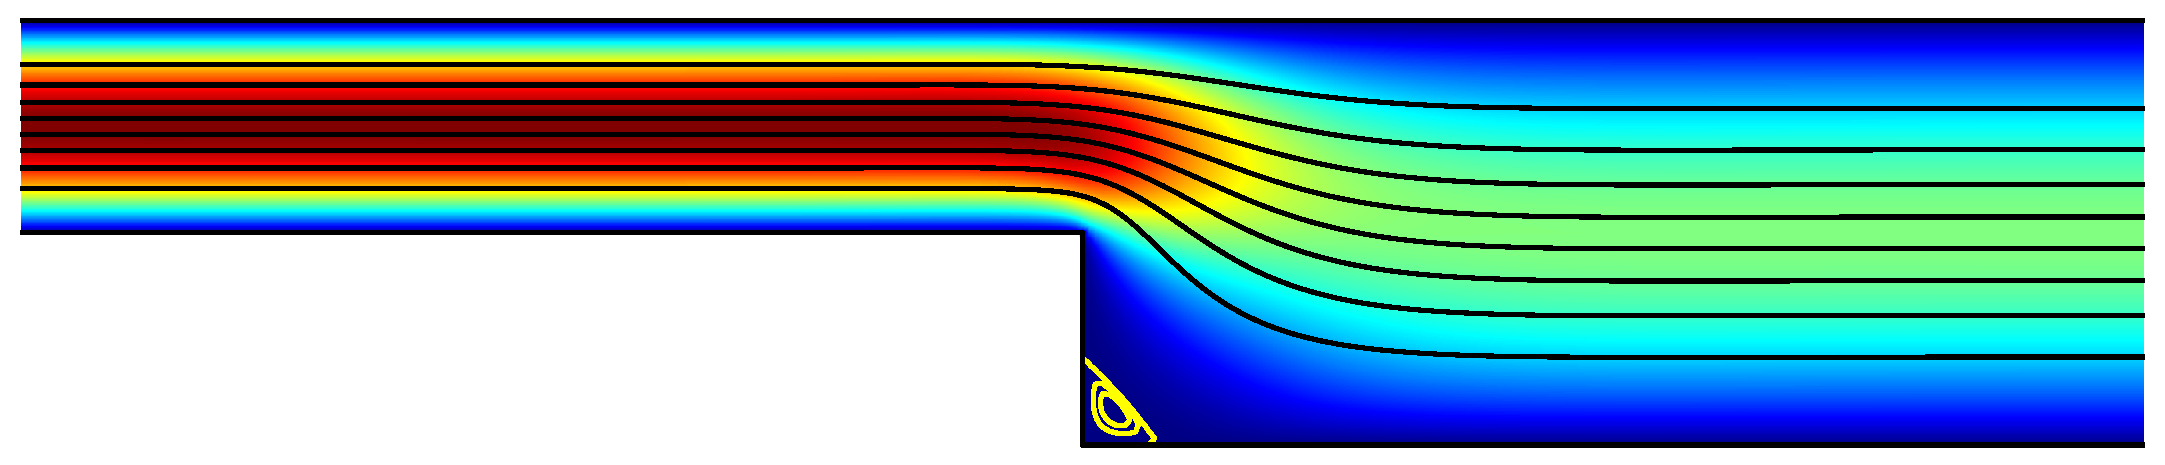
\includegraphics[width=\linewidth]{Figures/chan_soln}}
	\vfill
	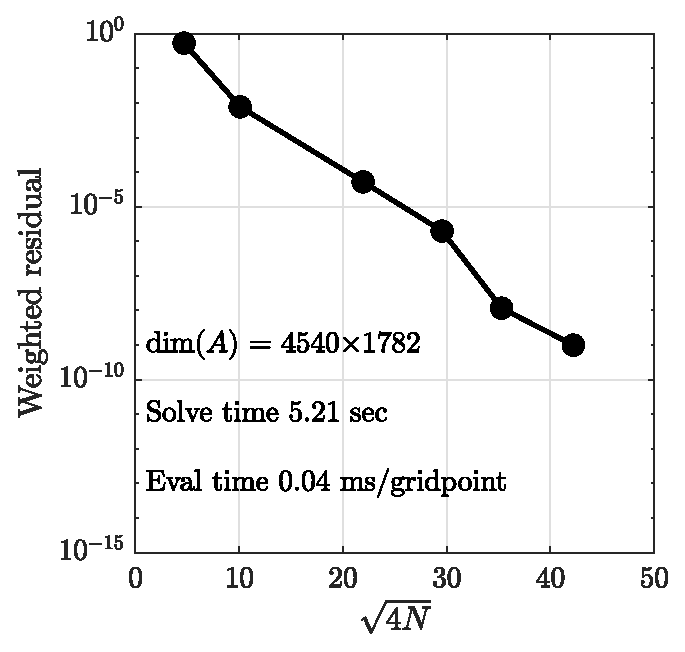
\includegraphics[height=0.3\linewidth]{Figures/chan_conv}
\end{figure}
\end{frame}


\begin{frame}
\frametitle{Infinite channel, flow past an obstacle}
\centering
\begin{figure}
	\subcaptionbox*{$-\infty\xleftarrow{\hspace*{0.4\linewidth}}x\xrightarrow{\hspace*{0.4\linewidth}}\infty$}{
	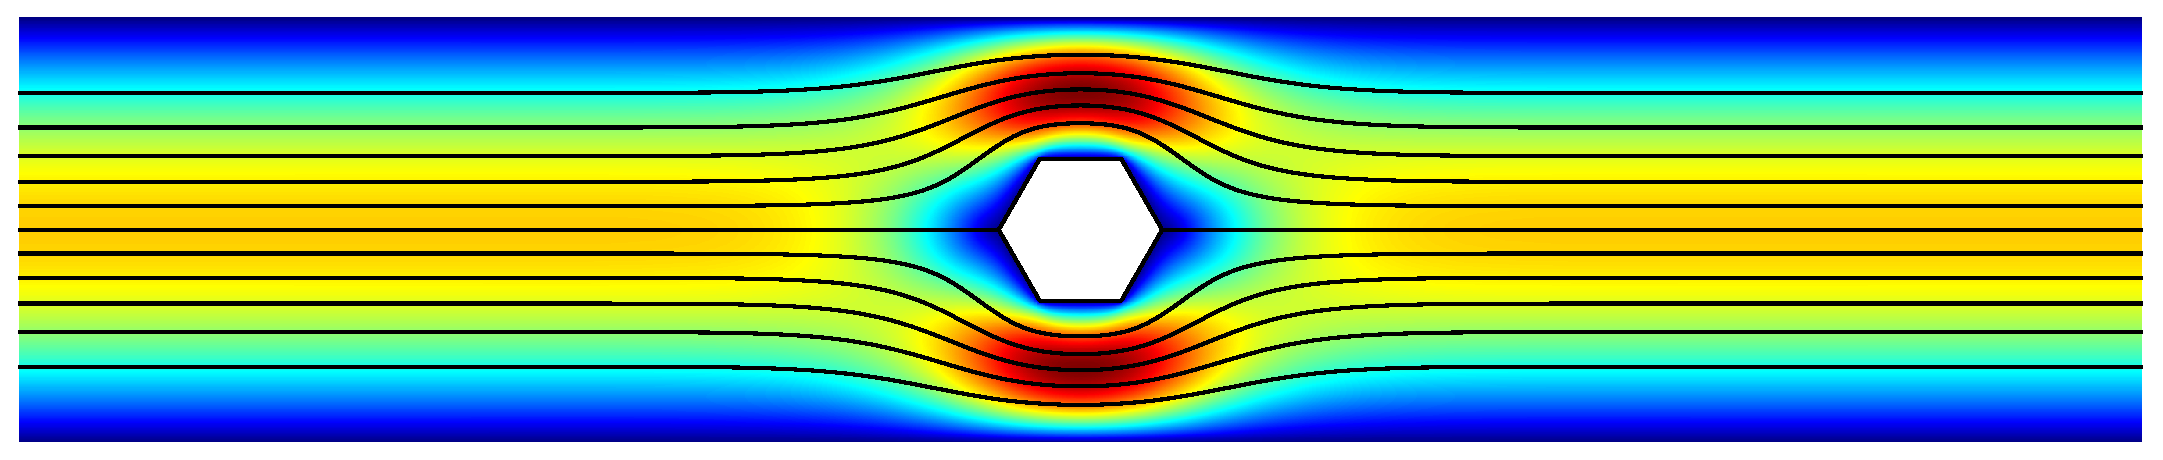
\includegraphics[width=\linewidth]{Figures/cyl_soln}}

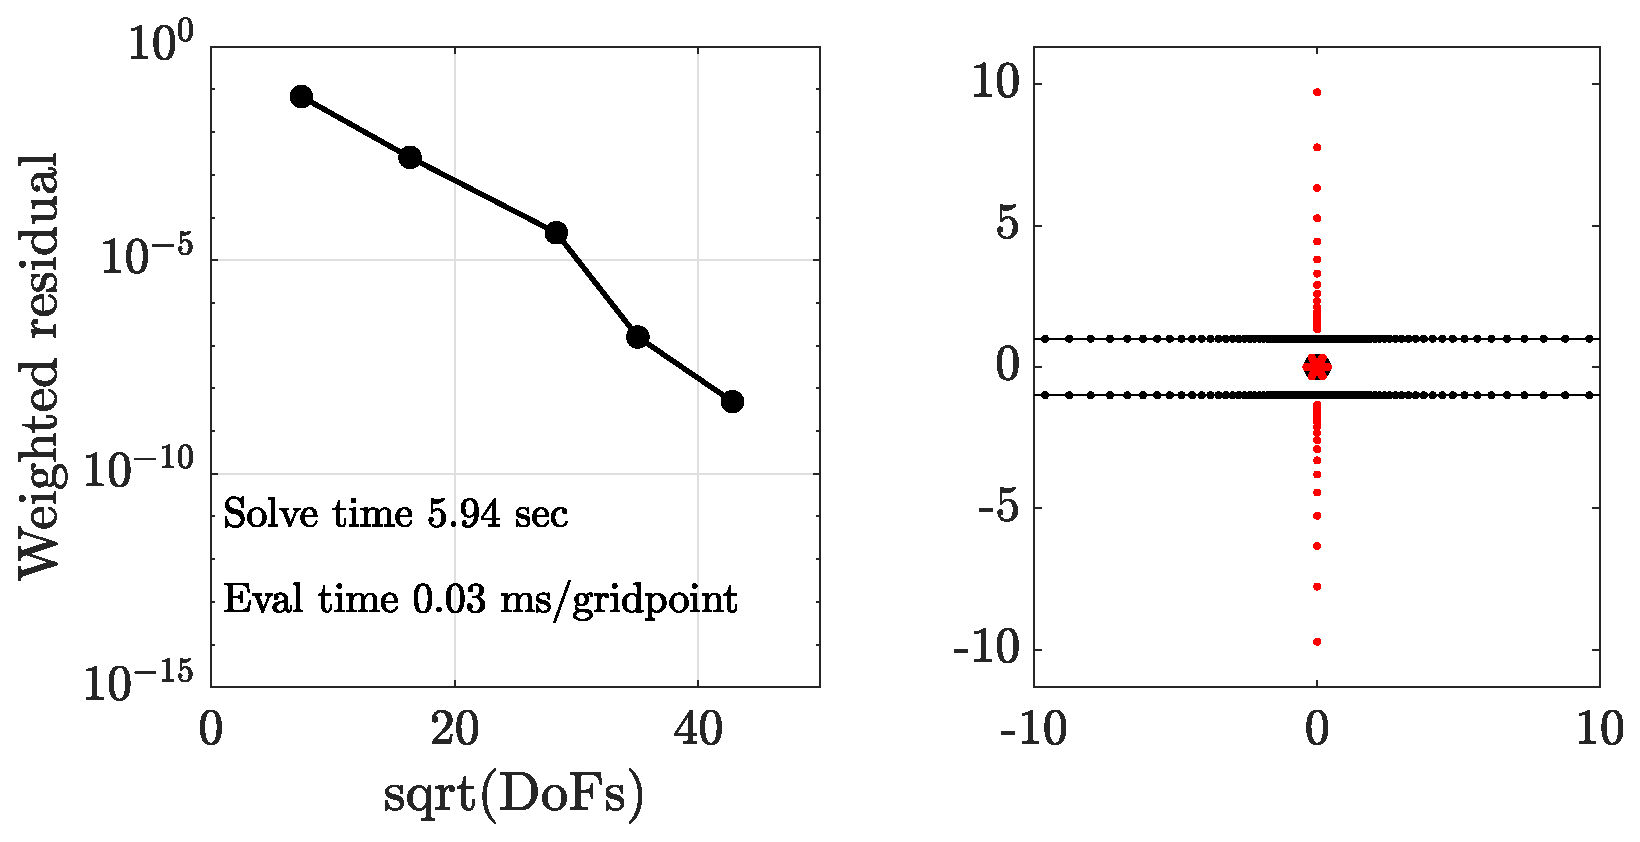
\includegraphics[height=0.3\linewidth]{Figures/cyl_conv}
\end{figure}
\end{frame}


\begin{frame}
\frametitle{Summary}
\begin{itemize}\itemsep 1em
\item Lightning Laplace for infinite and multiply connected regions
\item Lightning Stokes needs to solve for 2 analytic functions
\item Methods are computationally fast and converge root-exponentially
\end{itemize}

\bigskip
\textbf{Outlook}
\begin{itemize}\itemsep 1em
\item Multi-scale and domain decomposition approaches
\item Applications to linear elasticity
\end{itemize}

\end{frame}
%!TEX root = stokes_paper.tex

\section{Conclusion}

\bibliographystyle{plain}
\bibliography{references}
\end{document}